% *********************************************************************
% © 2021-2023 Jeremy Sylvestre
%
% Permission is granted to copy, distribute and/or modify this document
% under the terms of the GNU Free Documentation License, Version 1.3 or
% any later version published by the Free Software Foundation; with no
% Invariant Sections, no Front-Cover Texts, and no Back-Cover Texts. A
% copy of the license is included in the appendix entitled “GNU Free
% Documentation License” that appears in the output document of this
% PreTeXt source code. All trademarks™ are the registered® marks of
% their respective owners.
%
% *********************************************************************

\newcommand*{\xmin}{0}
\newcommand*{\xmax}{5}
\newcommand*{\ymin}{-3}
\newcommand*{\ymax}{5}

%
% DE is
%    dq/dt = r * (M - q) * q
% where we will take r = 1 and M = 4
%

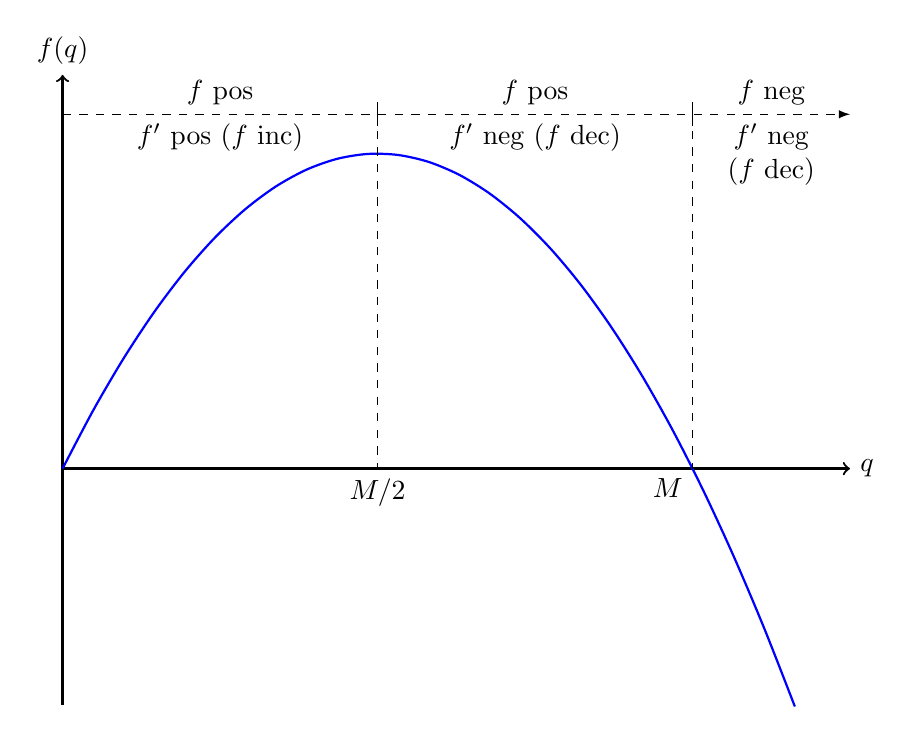
\begin{tikzpicture}
[
	closedpt/.style={circle,draw,fill,inner sep=0pt,minimum size=4pt},
	openpt/.style={circle,draw,inner sep=0pt,minimum size=4pt},
	xscale=2
]

	% axes
	\draw[->,thick] (0,0) -- (\xmax,0) node[right] {$q$};
	\draw[->,thick] (0,\ymin) -- (0,\ymax) node[above] {$f(q)$};

	\draw[thick,blue,smooth,domain=0:4.65] plot (\x, { 4 * \x - \x * \x });

	\draw[dashed] (2,4.5) -- (2,0) node[below] {$M/2$};
	\draw[dashed] (4,4.5) -- (4,0) node[below left] {$M$};

	\begin{scope}[yshift=4.5cm]

	\draw[dashed,-latex] (0,0) -- (\xmax,0);

	\draw (2,-0.15) -- (2,0.15);
	\node[above] at (1,0) {$f$ pos};
	\node[below] at (1,0) {$f'$ pos ($f$ inc)};

	\draw (4,-0.15) -- (4,0.15);
	\node[above] at (3,0) {$f$ pos};
	\node[below] at (3,0) {$f'$ neg ($f$ dec)};

	\node[above] at (4.5,0) {$f$ neg};
	\node[below,align=center] at (4.5,0) {$f'$ neg \\ ($f$ dec)};

	\end{scope}

\end{tikzpicture}
